%==============================================================================
% intervals.tex
%==============================================================================

\chapter{Intervals}
\label{cha:intervals}

Intervals \cite{Matsakis2009a} are a new, higher-level primitive for
parallel programming with which programmers directly construct the
program schedule. They are under active development at ETH Zurich as
part of the PhD research of Nicholas Matsakis \cite{Matsakis2010}.

\section{Introduction}
\label{sec:intervals-introduction}

[TODO: clean up]

Existing primitives for synchronizing the control-flow of parallel
threads, such as signals and barriers, are low-level and dangerous to
use. Like any low-level interface, they require careful attention to
implementation details to achieve good performance, and they are prone
to errors, particularly deadlocks and race conditions.

Intervals are a higher-level alternative that make parallel
programming safer while retaining the flexibility and efficiency of
threads. In the Intervals model, users create lightweight tasks and
order them using explicit happens before relations
\cite{Lamport1978}. Users need not specify when a thread should block
or acquire a lock: rather, they specify when a task should execute
relative to other tasks, and what locks it should hold when it
executes. The details of making this schedule come to pass are left to
the runtime system.

Because the intervals API supports arbitrary happens before relations,
the model is very flexible. Intervals can be used to emulate existing
thread primitives \cite{Matsakis2009a}, but they can also be used to
easily create program schedules for which no standard thread
primitives exist, such as peer-to-peer synchronization.

One of the primary goals in developing intervals is that program
errors should not lead to deadlocks. This includes both misuse of the
APIs but also miscellaneous errors which causes tasks to abort
unexpectedly, such as dereferencing a null pointer. A further goal is
that an error in one task should prevent other, dependent tasks from
executing.

\section{Model}
\label{sec:intervals-model}

[TODO: Clean up]

Intervals are first-class objects in the programming language that
represent the slice of program time used to achieve some
goal. Programmers create intervals explicitly and may also specify
ordering dependencies between them. Each interval has an associated
sequential subroutine called its task.

The conceptual model for intervals consists of points in time ordered
by a happens before relation. In the model, an interval \lstinline|i|
consists of a pair of points (\lstinline|i.start|, \lstinline|i.end|)
called the start and end point. The start point represents the moment
when the interval's task began to execute. The end point represents
the moment when the interval has conceptually finished. This is always
after the interval's task has returned. However, it may be delayed
further if there are predecessor points which happen before the end of
the interval. In that case, interval will not end until both its
predecessors have occurred and its task has finished.

\begin{figure}[htb]
  \centering
  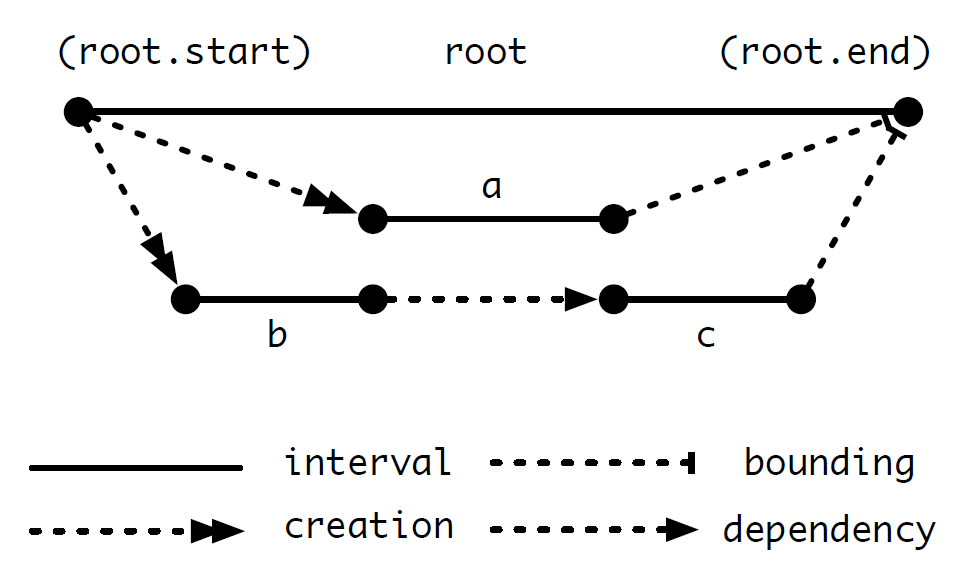
\includegraphics[scale=0.45]{intervals}
  \caption[Example interval graph]{Example interval graph: The nodes
    represent points in time. The transitive closure of all edges
    represents the happens before relation. The different kinds of
    edges indicate how the graph was constructed.}
  \label{fig:intervals}
\end{figure}

The interval model can be depicted as a graph, as shown in Figure
\ref{fig:intervals}. The points in time are represented as nodes in
the graph, and the happens before relation is shown by edges. The
different kinds of edges serve to distinguish how each edge was
created. All kinds of edges have the same meaning for the happens
before relation, but identifying how an edge was built also summarizes
the structure of the program which built the interval graph.

Interval edges connect the start and end points of an interval. We
generally label intervals but omit labels on the individual points; in
this graph, however, we included labels on the points of the
\lstinline|root| interval for illustrative purposes.

When the program begins, the graph consists only of an initial
interval, called root. As the program executes, it can create new
intervals by invoking functions in the API.  The interval i whose task
invoked the creation function is called the creator of the new
interval n. Every new interval is connected to its creator via a
creation edge from i.start to n.start, indicating that i must have
started in order for it to invoke the function which creates n. In
Figure 1, the interval root created all the others. We often omit
creation edges that do not affect the happens before relation, such as
the edge to interval c.

When creating a new interval n, the user must specify a bound point
p. Intervals working towards a common goal are generally given the
same bound. In terms of the happens before relation, bounds come after
the end of the interval, and so a bounding edge in the graph leads
from n.end to p.  Redundant bounding edges are sometimes omitted (as
with the interval b).

All the edges so far were constructed implicitly as a side effect of
constructing an interval. Users can also add arbitrary dependency
edges into the graph to reflect data dependencies or other
constraints. The only limitation is that the resulting schedule must
be acyclic. This permits very fine-grained control of the execution
order.

\section{Java API}
\label{sec:intervals-java-api}

Listing \ref{lst:intervals-example} contains Java code which uses the
Intervals API to construct the graph shown in figure
\ref{fig:intervals}.

\begin{lstlisting}[
  style=Float, 
  caption={[Intervals Java API example] Code to produce the sample interval graph shown in figure \ref{fig:intervals}},
  label=lst:intervals-example
]
public class Example extends Interval {
  public Example(Dependency dep, String name) {
    super(dep, name);
  }

  @Override
  protected void run() {
    // Task
  }
  
  public static void main(String[] args) {
    Intervals.inline(new VoidInlineTask() {
      public void run(Interval root) {
        Example a = new HB(root, "a");
        Example b = new HB(root, "b");
        Example c = new HB(root, "c");
        
        Intervals.addHb(b, c); //* \label{lst:intervals-example-add-hb}
        Intervals.schedule(); //* \label{lst:intervals-example-schedule}
      }
    });
  }
}
\end{lstlisting}

\subsection{Creating Intervals}
\label{sec:intervals-creating-intervals}

[TODO: Inheriting from Interval and implementing the run() method]

[TODO: Inline intervals]

\subsection{Scheduling Intervals}
\label{sec:intervals-scheduling-intervals}

[TODO: clean up]

Newly constructed intervals become eligible for execution once the
method \lstinline|schedule()| is invoked, as shown on line
\ref{lst:intervals-example-schedule} in Listing
\ref{lst:intervals-example}. This gives the user the opportunity to
construct any required dependencies or perform other
initialization. For example, adding the edge 
\lstinline|b $\rightarrow$ c| on line
\ref{lst:intervals-example-add-hb} would be unsafe if \lstinline|c|
could begin immediately, as it would be possible that
\lstinline|c.start| had already occurred before the call to
\lstinline|addHb()| could add the new dependency.

Explicit calls to \lstinline|schedule()| are unusual, however. This is
because the runtime automatically invokes \lstinline|schedule()| when
the \lstinline|run()| method of an interval's task returns.

\section{Interval Scheduler}
\label{sec:intervals-interval-scheduler}

[TODO: clean up]

In the background, an interval program relies on a scheduler that
respects the dependencies which the user specifies. The scheduler can
start an interval any time after the points which come before its
start have already occurred. If there is no path leading from one
point to another, then the two points are considered unordered. This
means that the scheduler would be free to order them any way it likes.

When an interval is created, it is also given a task to execute. When
the scheduler determines that all incoming dependencies on the
interval's start point have been resolved, it will arrange for that
task to execute. The end point of the interval occurs once the
interval's associated task has terminated and all incoming
dependencies on the end point are resolved.

%%% Local Variables: 
%%% mode: latex
%%% TeX-master: "thesis"
%%% End: 
